% ******************************************************** %
%              TEMPLATE DE INFORME                         %
% ******************************************************** %
% ******************************************************** %
%                                                          %
% ALGUNOS PAQUETES REQUERIDOS (EN UBUNTU):                 %
% ========================================
%                                                          %
% texlive-latex-base                                       %
% texlive-latex-recommended                                %
% texlive-fonts-recommended                                %
% texlive-latex-extra?                                     %
% texlive-lang-spanish (en ubuntu 13.10)                   %
% ******************************************************** %


\documentclass[a4paper]{article}
\usepackage[spanish]{babel}
\usepackage[utf8]{inputenc}
\usepackage{charter}   % tipografia
\usepackage{graphicx}
\usepackage[table,xcdraw]{xcolor}
\usepackage{hyperref}
%\usepackage{makeidx}
\usepackage{paralist} %itemize inline
\usepackage{algpseudocode}

\usepackage{float}
\usepackage{amsmath, amsthm, amssymb}
\usepackage{amsfonts}
%\usepackage{sectsty}
%\usepackage{charter}
%\usepackage{wrapfig}
\usepackage{listingsutf8}

% \setcounter{secnumdepth}{2}
\usepackage{underscore}
\usepackage{caratula}
\usepackage{url}
\usepackage{fixltx2e}

%\usepackage[superscript,biblabel]{cite}
%\usepackage{dibujitos}

% ********************************************************* %
% ~~~~~~~~              Code snippets             ~~~~~~~~~ %
% ********************************************************* %

\usepackage{color} % para snipets de codigo coloreados
\usepackage{fancybox}  % para el sbox de los snipets de codigo

\newcommand{\quotes}[1]{``#1''}


\definecolor{litegrey}{gray}{0.94}

\newenvironment{codesnippet}{%
	\begin{Sbox}\begin{minipage}{\textwidth}\sffamily\small}%
	{\end{minipage}\end{Sbox}%
		\begin{center}%
		\vspace{-0.4cm}\colorbox{litegrey}{\TheSbox}\end{center}\vspace{0.3cm}}

\definecolor{mygreen}{rgb}{0,0.6,0}
\definecolor{mygray}{rgb}{0.5,0.5,0.5}
\definecolor{mymauve}{rgb}{0.58,0,0.82}

\lstset{ %
  backgroundcolor=\color{litegrey},
  basicstyle=\footnotesize,
  breakatwhitespace=true,
  breaklines=true,
  captionpos=b,                    % sets the caption-position to bottom
  mathescape=true,
  keepspaces=true,
  language=Python,
  showspaces=false,
  tabsize=2,                       % sets default tabsize to 2 spaces
  inputencoding=utf8/latin1
}

\newcommand{\cuidado}{{\large $\Delta$!!!} \hspace*{1em}}

% ********************************************************* %
% ~~~~~~~~         Formato de las páginas         ~~~~~~~~~ %
% ********************************************************* %

\usepackage{fancyhdr}
\pagestyle{fancy}

\renewcommand{\sectionmark}[1]{\markright{\thesection\ - #1}}

\fancyhf{}

\fancyhead[LO]{Sección \rightmark} % \thesection\
\fancyfoot[LO]{\small{}} % alumnos
\fancyfoot[RO]{\thepage}
\renewcommand{\headrulewidth}{0.5pt}
\renewcommand{\footrulewidth}{0.5pt}
\setlength{\hoffset}{-0.8in}
\setlength{\textwidth}{16cm}
%\setlength{\hoffset}{-1.1cm}
%\setlength{\textwidth}{16cm}
\setlength{\headsep}{0.5cm}
\setlength{\textheight}{25cm}
\setlength{\voffset}{-0.7in}
\setlength{\headwidth}{\textwidth}
\setlength{\headheight}{13.1pt}

\renewcommand{\baselinestretch}{1.1}  % line spacing

% ******************************************************** %
% Cosas utiles
\newcommand\bigo{$\mathcal{O}$}

% ******************************************************** %

\begin{document}


\thispagestyle{empty}
\materia{Problemas, Algoritmos y Programación}
\submateria{Segundo Cuatrimestre de 2016}
\titulo{Trabajo Práctico 2}
\subtitulo{Grupo Bárbara liskov}

\maketitle
\newpage

\thispagestyle{empty}
\vfill

\thispagestyle{empty}
\vspace{2cm}
\tableofcontents
\normalsize

\vspace{4cm}
\section*{Puntajes}

\textbf{LLENAR}
\begin{center}
  \begin{tabular}{ | c | c | c | c| }
    \hline
    Ej1& Ej2 & Ej3 & Ej4 \\ \hline
     la & la & la & la \\ \hline
  \end{tabular}
\end{center}

\newpage
\section{Ejercicio 1}

\newcommand\sS{ \textbf{S} }
\newcommand\sT{ \textbf{T} }

En este problema queremos saber, dadas dos strings \sT y \sS, si \sS está contenida en \sT. Además queremos resolverlo en tiempo \bigo($|\sT|$).

\subsection{Algoritmo}

Implementamos el algoritmo KMP de búsqueda de substrings para poder resolver el problema en tiempo.
\\

Primero debemos definir lo que llamamos la \textit{tabla de bordes}. Un $borde$ de un string $s$ es un prefijo de longitud menor que a $|s|$ que también es sufijo de este. Nuestra tabla de bordes será un array de longitud $|\sS|$ donde en la posición $i$ nos indica el largo del mayor borde de $\sS[0..i)$.

    Para calcular la tabla vemos primero que el string vacío no tiene ningún borde, por lo que la primer posición de la tabla no tiene un valor definido, así que podemos setear $tabla[0] = -1$ (nos será útil luego). Además, el único prefijo de un string de largo $1$ será el string vacío, por lo que la $tabla[1] = 0$.

Para $i \geq 2$ si $b$ es un borde no vacío de $\sS[0..i)$, necesariamente $b[0.. \,|b|-1)$ era un borde $\sS[0..i-1)$ (no necesariamente el mayor) por lo que si queremos encontrar un borde de S[0..i) recorremos cada borde $b'$ de $i-1$ en orden decreciente hasta encontrar el primero tal que al agregarle un caracter se convierta en borde para $i$ (necesariamente el caracter a agregar será $\sS[ \,|b'|\, ]$, y será borde solo si el caracter es igual a $\sS[i-1]$).
No puede existir un borde de S[0..i) que no encontremos mediante este proceso, por la propiedad antes mencionada.
Si encontramos alguno, será el borde más grande de $i$, pues todos los bordes que podamos encontrar siguientes tendrán tamaño menor y $tabla[i] = |b'| + 1$. Si no se encuentra ninguno, el borde será el string vacío y $tabla[i] = 0$.

Ahora, en el paso anterior supusimos que podemos recorrer los bordes del prefijo $i-1$, pero no es tan directo ver que los tenemos en la tabla. Dado $i$ para el que queremos recorrer los bordes, conocemos el borde mayor $b_i$.

\begin{itemize}
    \item Si $b_i = 0$, no puede existir un borde menor.
    \item Si $b_i \neq 0$, sea $b_i'$ el segundo mayor borde. $b_i'$ existe porque siempre tenemos el borde vacío.

        Como $b_i$ y $b_i'$ son prefijos de $\sS[0..i)$ y $|b_i| > |b_i'|$, necesariamente $b_i'$ es un prefijo de $b_i$. Lo mismo vale como sufijos, por lo tanto sabemos que $b_i'$ es borde de $b_i$.
        Además vale la recíproca. Si tenemos un $b_i'$ cualquiera borde de $b_i$, es prefijo y es sufijo de un prefijo y sufijo de S[0..i), por lo cual es también prefijo y sufijo, lo que nos dice que un borde de un borde, tambien es borde.

        Y si hubiera un borde de $b_i$ de tamaño mayor a $|b_i'|$, por el razonamiento anterior sería también un borde de $\sS[0..i)$ y violaría nuestra suposición de que $b_i'$ es el segundo mayor borde. Por lo tanto $b_i'$ es el mayor borde de $b_i$, y ya lo tenemos calculado en $tabla[ \,|b_i|\, ]$.

        Se sigue entonces que podemos reproducir todos los bordes para $i$ en orden decreciente siguiendo la cadena $(tabla[i], \; tabla[tabla[i]], \; \ldots)$ hasta llegar al borde de largo 0, el string vacío.

\end{itemize}

\vspace*{1em}

Ahora que tenemos la tabla de bordes, queremos realizar la búsqueda de \sS en \sT.
\\

La idea es recorrer las posiciones $p$ de \sT en orden creciente (con $p \leq |\sT| - |\sS|$ pues \sS debe caber en lo que resta de \sT), decidiendo si el substring de tamaño $|\sS|$ a partir de esa posición es efectivamente igual a \sS. Para ello debemos recorrer cada caracter $i$-ésimo de \sS y compararlo con el caracter $p+i$ de \sT.

\begin{itemize}
    \item Si todos los caracteres de \sS matchean, entonces \sS es substring de \sT.

    \item Si la comparación con $\sS[i]$ falla (y las anteriores no), sabemos que \sS no comenzaba en la posición $p$ de \sT. Pero tenemos mas información que eso, ya que sabemos que $\sT[p..p+i) = \sS[0..i)$.

        Supongamos que \sS era substring de \sT comenzando desde la posición $p+j$ para algún $0 < j < i$. Por lo tanto, $\sT[p+j..p+i) = \sS[0..i-j) = \sT[p..p+i-j)$. Y entonces $\sS[0..i)$ tenía un borde de largo $i-j$ y como teníamos calculado la longitud del borde máximo, $tabla[i] \geq i-j \implies j \geq i - tabla[i]$.

        De esta forma sabemos que la siguiente posición candidato como inicio de \sS es $p + i - tabla[i]$ y además ya sabemos que $\sT[p + i - tabla[i].. p+i) = \sS[0..i - tabla[i])$, por lo que empezamos el nuevo escaneo con $i' = i - tabla[i]$.

        Es importante notar que como definimos $tabla[0] = -1$, en el paso anterior tendremos $0 - tabla[0] = 1$ y por lo tanto vale para $i=0$ si la nueva posición de escaneo la seteamos como $i' = max(0, i-tabla[i])$ (simplemente empezamos a escanear \sS desde la siguiente posición en \sT), por mas que el borde no esté propiamente definido.

\end{itemize}

\subsection{Pseudocódigo}

\begin{algorithmic}

\Function{precalcularTabla}{$s : string$}{$\; \rightarrow vector<int>$}
    \State $tabla : vector<int>$ de tamaño $|s|$
    \State $tabla$[$0$] $\gets -1$
    \State $tabla$[$1$] $\gets 0$
    \State $pos = 2$
    \State $prevBorde = 0$

    \While{$pos < |s|$}
        \If{$s[pos-1] = s[prevBorde]$}
            \State $prevBorde++$
            \State $tabla[pos] = prevBorde$
            \State $pos++$
        \ElsIf{$prevBorde > 0$}
            \State $prevBorde = tabla[prevBorde]$
        \Else
            \State $tabla[pos] = 0$
            \State $pos++$
        \EndIf
    \EndWhile

    \State \Return $tabla$
\EndFunction
\\

\Function{kmp}{$t : string, s : string$}{$\; \rightarrow bool$}
    \State $tabla = precalcularTabla(s)$
    \State $i = 0$
    \State $pos = 0$

    \While{$pos \leq |t|-|s|$}
        \If{$s[i] = t[i+pos]$}
            \If{$i = |s| - 1$}
                \State \Return $true$
            \EndIf
            \State $i++$
        \Else
            \State $pos = pos + i - tabla[i]$
            \State $i = max(0, tabla[i])$
        \EndIf
    \EndWhile

    \State \Return $false$
\EndFunction

\subsection{Complejidad}

Veamos primero la complejidad de $precalcularTabla$.

La inicialización de las variables se hace en \bigo($|s|$) ya que tenemos que crear el array.
Además vemos que el cuerpo del \textbf{while} se realiza en \bigo(1) por lo que nos queda analizar la cantidad de veces que se corre.

Lo importante es observar que en cada ciclo se incrementa $pos$ o $pos - prevBorde$, y ninguno de los dos decrementa nunca.

\begin{itemize}
    \item Si entra al \textbf{if}, $pos$ se incrementa en 1 y $pos - prevBorde$ se mantiene constante.
    \item Si entra al \textbf{else if}, $prevBorde$ se reemplaza por su borde mas grande, que es estrictamente menor. Por lo tanto $pos$ se mantiene constante y $pos - prevBorde$ incrementa.
    \item Si entra al \textbf{else}, $pos$ y $pos - prevBorde$ se incrementan.
\end{itemize}

Ahora, $pos$ está acotado por $|s|$ y como $prevBorde$ es siempre positivo, $pos - prevBorde$ también esta acotado por lo mismo. Por lo tanto el \textbf{while} no puede ejecutarse mas de $2 * |s|$ veces, por lo que se realiza en \bigo($|s|$).

Y si sumamos ambas complejidades, $precalcularTabla$ corre en \bigo($|s|$).

\vspace{1em}

Veamos ahora $kmp$ en sí.

Como por enunciado que la longitud de \sS es menor a la de \sT, \bigo($|\sS|$) $\in$ \bigo($|\sT|$), y por lo tanto la inicialización de variables se realiza en \bigo($precalcularTabla(\sS)$) $=$ \bigo($|\sT|$).

Vemos que el cuerpo del \textbf{while} se realiza en \bigo(1), por lo nuevamente que nuevamente queremos acotar la cantidad de ciclos. Para ello vamos a ver que en cada ciclo se incrementa $pos$ o $pos + i$, y nunca se decrementan.

\begin{itemize}
    \item Si entra al primer \textbf{if} y no termina (no entra el segundo \textbf{if}), $pos + i$ se incrementa en 1 y $pos$ se mantiene constante.
    \item Si entra al \textbf{else}, $pos$ se incrementa ya que si i es mayor a 0, $i - tabla[i]$ equivale a $i - |mayor borde de i|$ que es necesariamente positivo, y si $i=0$ la resta vale 1 (por como generamos la tabla). Por otro lado si $i>0$, $pos + i$ se mantiene constante y si $i$ era 0 se incrementa en 1.
\end{itemize}

Finalmente, vemos que $pos \leq |\sT| - |\sS|$ y $i < |\sS|$ por lo que el \textbf{while} se ejecutará a lo sumo $cota\ pos + cota\ (pos+i) \;\in\; \bigo(|\sT|) + \bigo(|\sT|) = \,\bigo(|\sT|)$ veces.

Por lo tanto, el algoritmo completo tendrá complejidad temporal en \bigo($|\sT|$).

\end{algorithmic}


\newpage
\section{Ejercicio 2}

\subsection{Enunciado}

\par{El enunciado nos dice que tenemos un grupo de A acciones, cuyos precios conocemos en D días. 
Vamos a agrupar las acciones en gráficos. Dos acciones pueden ir en un mismo gráfico, si las lineas de sus dibujos
como función no se tocan en ningún punto.}
\par{Nos piden que demos la mínima cantidad de gráficos necesaria para poder graficar todas las acciones, con 
la restricción previamente mencionada.} 

\subsection{¿Cuándo se cruzan dos acciones?}

\par{Vamos a notar que, el hecho de que dos acciones \textbf{NO} se crucen es equivalente a que 
haya una cuyos precios en los D días sean estrictamente mayores a los correspondientes de la otra.}

\par{Que dos acciones se crucen significa que, si tenemos un segmento A $\rightarrow$ B de una acción, 
y otro C $\rightarrow$ D de la otra y correspondientes al mismo día,  entonces A mayor a C y B menor a D, o viceversa.} 

\par{Si en los D días, una acción siempre domina a la otra (decimos que una ``está arriba'' de la otra ), entonces trivialmente no se cruzan.}

\par{Si no se cruzan, entonces no hay dos segmentos correspondientes al mismo día que se den vuelta. 
O A mayor a C y B mayor a D, o la inversa. Entonces una acción esta arriba de la otra. Afirmamos entonces que son equivalentes.}

\subsection{Definamos un orden}

\par{Nos interesa notar algunas propiedades de la relación \textbf{estar arriba}. Para empezar, 
la relación es transitiva. Si A está arriba de B, y B de C, A está arriba de C.
Si con un poco de cuidado, permitimos que dos elementos estén relacionados si sus precios son iguales en todo momento, entonces
la relación nos queda reflexiva y antisimétrica. Con lo cual, nos define un \textbf{orden parcial}. }

\par{Lo que el problema nos pide es una cantidad mínima de gráficos que necesitamos para dibujar todas las acciones. 
Por la equivalencia que vimos antes, gráficos de este estilo, son conjuntos de acciones donde no se cruzan, es decir, 
una esta arriba de otra, para dos cualesquiera del conjunto. Y como la relación es transitiva, existe una acción,
A$_1$ $>$ A$_2$ $>$ ... $>$ A$_k$, en un conjunto del mismo gráfico, con k acciones.} 

\subsection{La gallinita dijo Eureka}

\par{Por la observación, vemos que lo que estamos buscando es la mínima cantidad de \textbf{cadenas} que necesitamos
para cubrir un conjunto parcialmente ordenado. Donde una cadena, es un conjunto totalmente ordenado.}

\par{Sabemos además por el \textbf{Teorema de Dilworth} que esta mínima cantidad de cadenas es igual a la mínima anticadena
(un conjunto de elementos incomparables), y que estas se pueden calcular mediante un Flujo Máximo!}

\par{Usamos esta construcción de grafo de Dilworth, para calcular la mayor anticadena. El grafo que nos queda 
tiene para cada acción a $\in$ Acciones, dos nodos a$'$, a$''$ $\in$ V. Por otro lado, tenemos dos nodos, s y t (source y sink del nuevo grafo).
s esta conectado con todos los a$'$, con aristas de capacidad 1. Y t esta conectado con todos los a$''$ con aristas de capacidad 1.
Por último, todos los si tenemos dos acciones a,b y a \textbf{está arriba} de b, entonces a$'$ esta conectada con b$''$ con una arista de capacidad 1.
Si f es un flujo máximo de s a t en este nuevo grafo, por el teorema de Dilworth, la mayor anticadena es igual a $|acciones| - |f|$ = $A - |f|$, y es lo que buscábamos.  
}

\subsection{Complejidad}

\par{La primer parte de nuestra solución, para construir el grafo, necesita ver si dadas dos acciones, 
una esta arriba de la otra. Dadas dos acciones, chequear esto nos tarda \bigo(D), simplemente iterando por los días.
Por eso esta primer parte es \bigo($A^2 \times D $)}

\par{Luego, tenemos que buscar el flujo máximo. Utilizamos el algoritmo de Edmonds-Karp, que en cada iteración hace un BFS.
Pero utilizamos la cota que nos dice que la cantidad de iteraciones esta acotada por el flujo máximo. 
El flujo máximo es A, por construcción del grafo (las aristas que salen de s).
Entonces sabemos que la complejidad del algoritmo es \bigo($ (E + V) \times A$), donde E y V son las aristas y nodos respectivamente.
Además estas son \bigo($A^2$) y \bigo($A$) respectivamente, por lo cual el algoritmo de flujo termina siendo \bigo($ (A^2 + A) \times A$) 
= \bigo($ (A^2) \times A$). }

\par{Entonces, en total todo el algoritmo es \bigo($ A^2 \times (A + D) $) que es exactamente lo pedido.}


\subsection{Pseudocódigo}
	
\begin{algorithmic}
\Function{calcular$\_$camino$\_$aumento}{capacidad_red_residual, G, source, sink}
	\State cola c, visited[tamaño(G)] = [false .. false], padre[tamaño(G)] = [-1 .. -1]
	\State c.encolar(source)
	
	\Comment{BFS}

	\While{not cola.vacia}
		\State actual $\leftarrow$ cola.tope()
		\State cola.desencolar
		
		\State visited[actual] $\leftarrow$ true
	
		\For{v : adj[actual]} \Comment{Para cada vecino del nodo actual en G}
				\If {not visited[v] and capacidad_red_residual[actual][v] == 1}
					\State p[v] $\leftarrow$ actual
					\State cola.encolar(v)
				\EndIf
		\EndFor 
	\EndWhile

	\If{not visited[sink]} 
		\State \Return 0 \Comment{Si no hubo camino de aumento (no llegué al nodo final)}
	\EndIf

	\Comment{Caso contrario reconstruyo el camino y reconstruyo la capacidad de la red residual.}
	\State actual $\leftarrow$ sink
	\State padre $\leftarrow$ p[actual]
	
	\While{padre!=-1}
		\State capacidad_red_residual[padre][actual] $\leftarrow$ 0
		\State capacidad_red_residual[actual][padre] $\leftarrow$ 1
		
		\State actual $\leftarrow$ padre
		\State padre $\leftarrow$ p[actual]
	\EndWhile

	\State \Return 1 \Comment{Toda arista tiene capacidad 1.}
\EndFunction
\end{algorithmic}
\hspace{1cm}

\begin{algorithmic}
\Function{flujo$\_$máximo}{capacidad_red_residual, G,source, sink}
	\State flujo$\_$total $\leftarrow$ 0
	\Repeat 
			\State aumentar $\leftarrow$ calcular$\_$camino$\_$aumento(capacidad_red_residual, G, source,sink)
			\State flujo$\_$total = flujo$\_$total + aumentar
	\Until{aumentar $\neq$ 0}
	
\EndFunction
\end{algorithmic}
\hspace{1cm}

\begin{algorithmic}
\Function{conectar}{capacidad_red_residual, G, A, B}
	\State capacidad_red_residual [a][b] $\leftarrow$ 1
	\State conectar A con B en G
	\State conectar B con A en G
\EndFunction
\end{algorithmic}
\hspace{1cm}


\begin{algorithmic}
\Function{está_arriba_de}{a, b, D, precios[][]}
	\For{ i $\leftarrow$ [1 .. D]}
		\If{precios[a][i] $\leq$ precios[b][i]}
			\State \Return false
		\EndIf
	\EndFor	
	\State \Return true
\EndFunction
\end{algorithmic}
\hspace{1cm}

\begin{algorithmic}
\Function{main}{A, D, precios [][]}
	\State \textit{\textbf{La red residual será modelada como una matriz de Tamaño(G) * Tamaño(G)}}
	\State \textit{\textbf{Y como las capacidades en la red residual 0 o 1, entonces al generar caminos de aumento se simplificará para que devuelva 1 de aumento en el flujo si hay camino y 0 caso de que no.}}
	\State \textit{\textbf{El grafo como una lista de adyacencia.}}
	\State Tamaño(G) = 2 * A + 2
	\State capacidad_red_residual [Tamaño(G)][Tamaño(G)] $\leftarrow$ [0 .. 0] 
	\State source $\leftarrow$ 0, sink $\leftarrow$ 2*A+1

	\For{v $\leftarrow$ [1..A]}
		\State conectar(capacidad_red_residual, G, source, v$'$) \Comment{Conecto al source con los nodos del conjunto A.}
		\State conectar(capacidad_red_residual, G, v$''$, sink) \Comment{Conecto a los nodos del conjunto B con el sink.}
	\EndFor

	\For{ v $\leftarrow$ [1..A]}
		\For{w $\leftarrow$ [1..A]}
			\If{v $\neq$ w and esta_arriba(v, w, D, precios)} 
				\State conectar(capacidad_red_residual, G, v$'$, w$''$)
			\EndIf
		\EndFor
	\EndFor
	
	\Return A - flujo$\_$máximo(capacidad_red_residual, G, source, sink)

\EndFunction

\end{algorithmic}



\newpage
\section{Ejercicio 3}

En este ejercicio nos dan una matriz de sueldos correspondientes a cada posible cargo y antigüedad que puede tener un docente. A partir del cargo y antigüedad de un docente, lo que cobra es equivalente a $\sum_{i = 1}^{cargo} \sum_{j = 1}^{antiguedad} sueldos[i][j]$. Ahora bien un docente siempre tiene aspiraciones más altas con lo cual a pesar de tener un cargo c$_1$ y una antigüedad a$_1$, en realidad aspira a tener cargo c$_2$ y antigüedad a$_2$. \newline

Lo que le interesa saber es el monto de lo que cobraría si tuviera cargo c$_2$ y antigüedad a$_2$, que no podría conseguir si mantuviera su cargo c$_1$ (pudiendo aumentar su antigüedad hasta a$_2$) o si bien mantuviera su antigüedad (pudiendo subir de cargo hasta c$_2$). Vamos a asumir que a$_2$ y c$_2$ siempre son mayores o iguales a a$_1$ y c$_1$ respectivamente, la antigüedad de por sí no puede bajar, y no tiene demasiado sentido que un docente aspire a tener un peor cargo. \newline

Es decir, lo que nos interesa calcular es $\sum_{i = 1}^{c_2} \sum_{j = 1}^{a_2} sueldos[i][j]$ menos lo que gana actualmente y lo que podría ganar si mantiene fijo el cargo y sube su antigüedad o si mantiene fijo la antigüedad y sube el cargo (sin pasarse de c$_2$ ni de a$_2$). En términos de la matriz de sueldos, tenemos: 

\begin{enumerate}
	\item Lo que ganaría con cargo c$_2$ y antigüedad a$_2$ : $\sum_{i = 1}^{c_2} \sum_{j = 1}^{a_2} sueldos[i][j]$
	\item Lo que gana actualmente con cargo c$_1$ y antigüedad a$_1$ : $\sum_{i = 1}^{c_1} \sum_{j = 1}^{a_1} sueldos[i][j]$
	\item Lo que puede ganar como máximo manteniendo cargo c$_1$ pero subiendo antigüedad :

	 $\sum_{i = 1}^{c_1} \sum_{j = 1}^{a_2} sueldos[i][j]$
	\item Lo que puede ganar como máximo manteniendo antigüedad a$_1$ pero subiendo cargo : 

	$\sum_{i = 1}^{c_2} \sum_{j = 1}^{a_1} sueldos[i][j]$
\end{enumerate}

En definitiva, lo que queremos es la primera $-$ la unión de las otras 3. El problema por un lado es que la tercera y cuarta incluyen a la segunda ($a_2 \geq a_1\ y\ c_2 \geq c_1$) y por otro, la intersección de la tercera y la cuarta es efectivamente la segunda. Con lo cual no podemos realizar la resta de una, ya que estaríamos restando algunos sueldos múltiples veces. Hay varias formas de resolver esto. \newline

Una de ellas sería hacer que cada conjunto sea independiente, para que no haya posibilidad de estar restando lo mismo múltiples veces. Esto sería hacer $\sum_{i = 1}^{c_2} \sum_{j = 1}^{a_2} sueldos[i][j]$ - $\sum_{i = 1}^{c_1} \sum_{j = 1}^{a_1} sueldos[i][j]$ - $\sum_{i = c_1}^{c_1} \sum_{j = a_1 + 1}^{a_2} sueldos[i][j]$ - $\sum_{i = c_1 + 1}^{c_2} \sum_{j = a_1}^{a_1} sueldos[i][j]$. La nombraremos la forma complicada.  \newline

Otra forma sería sumar lo que se repite, como para cancelar lo que resté múltiples veces. Esto sería hacer $\sum_{i = 1}^{c_2} \sum_{j = 1}^{a_2} sueldos[i][j]$ - $\sum_{i = 1}^{c_1} \sum_{j = 1}^{a_2} sueldos[i][j]$ - $\sum_{i = 1}^{c_2} \sum_{j = 1}^{a_1} sueldos[i][j]$ + $\sum_{i = 1}^{c_1} \sum_{j = 1}^{a_1} sueldos[i][j]$. La nombraremos la forma copada.  \newline

Otra forma sería calcular directamente lo que queremos, que es $\sum_{i = c_1 + 1}^{c_2} \sum_{j = a_1 + 1}^{a_2} sueldos[i][j]$. La nombraremos la forma ineficiente.

\subsection{Resolviendo el problema}

En definitiva, una posible solución es por cada una de las sumatorias que necesito, recorrer la matriz y sumar lo que necesito. Luego es cuestión de aplicar alguna de las cuentas mencionadas. El problema de esto es que la complejidad depende en el mejor de los casos (forma ineficiente) de $(c_2 - c_1) \times (a_2 - a_1)$. El sólo hecho de leer el input para guardar la matriz nos da $O(a \times c)$, mientras que la complejidad que nos piden es $O(a \times c + q)$. Si por cada pregunta calculamos la respuesta en $O((c_2 - c_1) \times (a_2 - a_1))$, no nos daría la complejidad requerida.  \newline

Lo que vamos a buscar hacer es resolver cada pregunta en O(1). Para hacer esto, en vez de guardarnos la matriz de los sueldos, en la posición (i, j) vamos a guardarnos la sumatoria de los sueldos con cargo menor o igual a i y antigüedad menor o igual a j. Es decir, $\sum_{i = 1}^{i} \sum_{j = 1}^{j} sueldos[i][j]$. Si pudiésemos realizar esto en $O(a \times c)$, podríamos usar la forma complicada y tener tanto $\sum_{i = 1}^{c_2} \sum_{j = 1}^{a_2} sueldos[i][j]$ como $\sum_{i = 1}^{c_1} \sum_{j = 1}^{a_1} sueldos[i][j]$ en O(1), mientras que $\sum_{i = c_1}^{c_1} \sum_{j = a_1 + 1}^{a_2} sueldos[i][j]$ y $\sum_{i = c_1 + 1}^{c_2} \sum_{j = a_1}^{a_1} sueldos[i][j]$ lo podría calcular recorriendo la matriz original en $O((c_2 - c_1) + (a_2 - a_1))$.  \newline

Pero queremos O(1). Podríamos ver cómo calcular las 2 otras partes en O(1), o bien usar la forma copada que son todas cuentas con ambos índices empezando en 1, que son datos que tengo en mi matriz. $\sum_{i = 1}^{c_2} \sum_{j = 1}^{a_2} sueldos[i][j]$ es equivalente a mi nueva matriz en la posición (c$_2$, a$_2$), $\sum_{i = 1}^{c_1} \sum_{j = 1}^{a_2} sueldos[i][j]$ en la posición (c$_1$, a$_2$), $\sum_{i = 1}^{c_2} \sum_{j = 1}^{a_1} sueldos[i][j]$ en la posición (c$_2$, a$_1$) y $\sum_{i = 1}^{c_1} \sum_{j = 1}^{a_1} sueldos[i][j]$ en la posición (c$_1$, a$_1$). Es decir, accediendo a la matriz en O(1), podría hacer esas 3 cuentas (1 sumas y 2 restas) en O(1) y así cumplir con lo requerido.  \newline

Resta ver entonces cómo formar la matriz que quiero de las sumatorias en $O(a \times c)$. Para hacer esto, lo que vamos a hacer es ir recorriendo la matriz original en orden izquierda a derecha, abajo hacia arriba. Es decir, nos movemos por las columnas y al llegar a la última, avanzamos de fila y volvemos a empezar con las columnas. Veamos que si quiero calcular lo que debo poner en (i, j), eso es equivalente a lo que había en la matriz original en (i, j) + la matriz en (i, j - 1) + la matriz en (i - 1, j) - la matriz en (i - 1, j - 1).  \newline

Por el orden en que voy calculando, lo que hay arriba y a la izquierda ya lo tengo calculado, con lo cual tengo la información que necesito ya calculada. Veamos por ejemplo que queremos calcular la posición (4, 4).

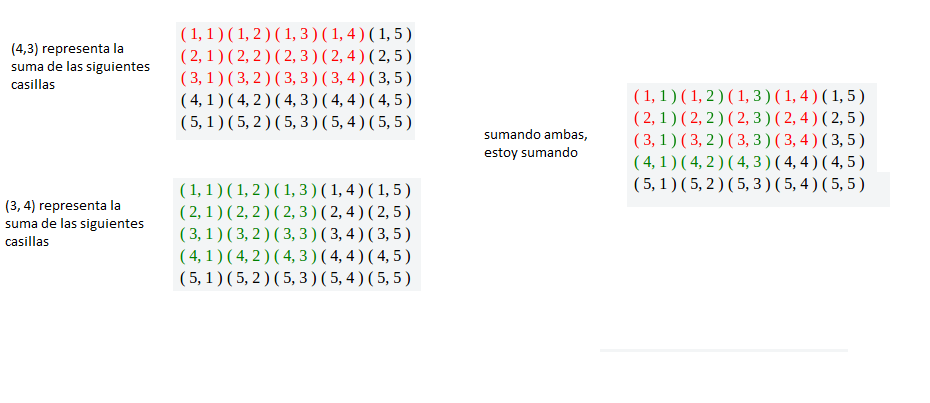
\includegraphics[scale=0.5]{img/tabla.jpg}

Como puede verse en el dibujo, si sumo lo que hay en la matriz en (i, j - 1) + lo que hay en la matriz en (i - 1, j), estoy sumando la intersección 2 veces. Esta intersección corresponde a lo que hay en la matriz en (i - 1, j - 1). Con lo cual si hago M(i, j - 1) + M(i - 1, j) - M(i - 1, j - 1), estoy sumando cada parte 1 sola vez, y luego sólo resta sumarle el valor del sueldo en la matriz original en la posición (i, j) para tener lo que quería : la sumatoria de lo que hay arriba y a la izquierda, incluyendo (i, j). \newline

Una vez obtenida esta matriz, puedo resolver cada pregunta en O(1), basta con hacer la cuenta mencionada en la forma copada. Como cada pregunta la resolvemos en O(1) y hay q preguntas, y como para armar la matriz simplemente hago 4 accesos a matriz, 2 sumas y 1 resta por cada posición, es O(1) para calcular cada posición y hay $a \times c$ posiciones, con lo cual la complejidad de resolver el problema me queda O ($a \times c + q$), cumpliendo con lo pedido.

\subsection {Detalles de implementación}

Como para calcular una posición de la matriz accedo a (i, j - 1),  (i - 1, j) y (i - 1, j - 1), es posible que en los casos borde (los bordes de arriba y a la izquierda de la matriz) alguna de estas posiciones no exista. Con lo cual, habría que hacer las sumas y restas correspondientes sólo si existen esas posiciones en la matriz. Para evitar estos chequeos, lo que hacemos es en vez de tener una matriz de $a \times c$, tenemos una matriz de $(a + 1) \times (c + 1)$ (que no modifica la complejidad) como para que nos \quotes{sobre} los bordes de arriba y a la izquierda. \newline

En estos bordes colocamos todos 0, así después cuando haga las cuentas estas posiciones siempre existen y sumar o restar 0 si no había nada, es justamente lo que quería, el 0 es el elemento neutro de la suma y resta así que nos sirve para lo que queremos. Además de esta manera no tenemos que preocuparnos por que la matriz sea 0-indexed y las coordenadas que nos dan (cargo y antigüedad) con las preguntas son 1-indexed. De esta forma, no hay que estar restando 1 a las coordenadas que nos dan para pasarlo a 0-indexed.\newline

Otro detalle es que la matriz de las sumatorias se puede ir calculando a medida que leo el input, ya que el orden en que decidí calcular la matriz es el mismo orden en que leo el input. Sólo hay que tener cuidado de iniciar la primer fila y primer columna con 0 antes de leer el input para los casos borde mencionados. \newline

Hay que mencionar también que estamos suponiendo en la implementación que la suma de todos los sueldos no se pasa de lo que puede almacenar un int, de no ser así habría que usar long o lo necesario para que no suceda. Estamos suponiendo también que a$_2$ y c$_2$ son $\geq$ a$_1$ y c$_1$ respectivamente ya que entendimos que en este problema eso es lo más lógico.

\subsection {Pseudocódigo}

\begin{algorithmic}

	\State $matriz[cargos + 1][antiguedad + 1] \gets [0...0]$ \Comment{Inicializo una matriz con ceros por lo menos en la primer fila y primer columna}

	\For{c $\gets$ 1 .. cargos}
		\For{a $\gets$ 1 .. antigüedad}
			\State $matriz[c][a] \gets leer\_input()$
			\State $matriz[c][a] \gets matriz[c][a] + matriz[c - 1][a] + matriz[c][a - 1] + matriz[c - 1][a - 1]$
		\EndFor
	\EndFor

	\For{q $\gets$ 1 .. preguntas}
		\State $c_1, a_1, c_2, a_2 \gets leer\_input()$
		\State $res \gets matriz[c_2][a_2] - matriz[c_2][a_1] - matriz[c_1][a_2] + matriz[c_1][a_1]$
		\State mostrar(res)
	\EndFor

\end{algorithmic}

\newpage
\section{Ejercicio 4}


\end{document}
